%%%%%%%%%%%%%%%%%%%%%%%%%%%%%%%%%%%%%%%%%%%%%%%%%%%%%%%%%%%%%%%%%%% 
%%%%%%%%%%%%%%%%%%%%%%%%%%%%%%%%%%%%%%%%%%%%%%%%%%%%%%%%%%%%%%%%%%% 
%%%%%%%%%%%%%%%%%%%%%%%%%%%%%%%%%%%%%%%%%%%%%%%%%%%%%%%%%%%%%%%%%%% 
\begin{frame}
  \frametitle{Kokkos: a programming model for performance portability}

  \only<1>{
    \begin{itemize}
    \item \textcolor{blue}{\textbf{Kokkos}} is a \textbf{C++ library} with \textcolor{red}{\textbf{parallel algorithmic patterns}} AND \textcolor{red}{\textbf{data containers}} for \textcolor{blue}{\textbf{node-level parallelism}}.
    \item Implementation relies heavily on \textbf{meta-programing} to derive native low-level code (OpenMP, Pthreads, CUDA, ...) and adapt data structure memory layout at compile-time
    \item Core developers at \textcolor{violet}{\textbf{SANDIA NL}} (\textbf{H.C. Edwards, C. Trott})
    \end{itemize}
  }
  \only<2>{
    \begin{itemize}
    \item \textcolor{darkgreen}{\textbf{Open source}}, \myurl{https://github.com/kokkos/kokkos}
    \item Primarily developped as a base building layer for \textbf{generic high-performance parallel linear algebra} in \myhref{https://github.com/trilinos/Trilinos}{Trilinos}
    \item Also used in molecular dynamics code, e.g. \myhref{http://lammps.sandia.gov/}{LAMMPS}
    \item Goal: \textcolor{orange}{\textbf{ISO/C++ 2020 Standard}} subsumes Kokkos abstractions
    \end{itemize}
  }
  \begin{center}
    \includegraphics<1-2>[width=6cm]{doc/perf_portability/kokkos_summary}
  \end{center}

\end{frame}

%%%%%%%%%%%%%%%%%%%%%%%%%%%%%%%%%%%%%%%%%%%%%%%%%%%%%%%%%%%%%%%%%%% 
%%%%%%%%%%%%%%%%%%%%%%%%%%%%%%%%%%%%%%%%%%%%%%%%%%%%%%%%%%%%%%%%%%% 
%%%%%%%%%%%%%%%%%%%%%%%%%%%%%%%%%%%%%%%%%%%%%%%%%%%%%%%%%%%%%%%%%%% 
\begin{frame}
  \frametitle{Kokkos: a programming model for performance portability}

  {\large \textcolor{blue}{\textbf{Kokkos abstract concepts}}}

  \begin{itemize}
  \item \textbf{Execution patterns (what):}\\
    \textcolor{darkgreen}{parallel\_for, parallel\_reduce, ...}
  \item \textbf{Execution policy (how):}\\
    \textcolor{darkgreen}{range iterations, teams of threads, ...}
  \item \textbf{Execution space (where):}\\
    \textcolor{darkgreen}{OpenMP, PThreads, CUDA, numa, ...}
  \item \textbf{Memory space: data containers} with architecture adapted memory layout\\
    {\small \textcolor{darkgreen}{\texttt{Kokkos::View, Kokkos::DualView, Kokkos::UnorderedMap,...}}}
  \item \textbf{Memory layout:} (important for vectorization, memory coalescence, ...)\\
    \textcolor{darkgreen}{row-major, column-major, AoS, SoA, ...}\\
    $data(i,j,k)$ \textcolor{red}{architecture aware}.
  \end{itemize}
  
  {\scriptsize reference: \myhref{https://cfwebprod.sandia.gov/cfdocs/CompResearch/docs/2016-04-Kokkos-SIAM-PP.pdf}{Kokkos: Manycore programmability and performance portability, SIAM conference, Paris, 2016}}

\end{frame}

%%%%%%%%%%%%%%%%%%%%%%%%%%%%%%%%%%%%%%%%%%%%%%%%%%%%%%%%%%%%%%%%%%% 
%%%%%%%%%%%%%%%%%%%%%%%%%%%%%%%%%%%%%%%%%%%%%%%%%%%%%%%%%%%%%%%%%%% 
%%%%%%%%%%%%%%%%%%%%%%%%%%%%%%%%%%%%%%%%%%%%%%%%%%%%%%%%%%%%%%%%%%% 
\begin{frame}
  \frametitle{Kokkos: a programming model for performance portability}

  \begin{center}
    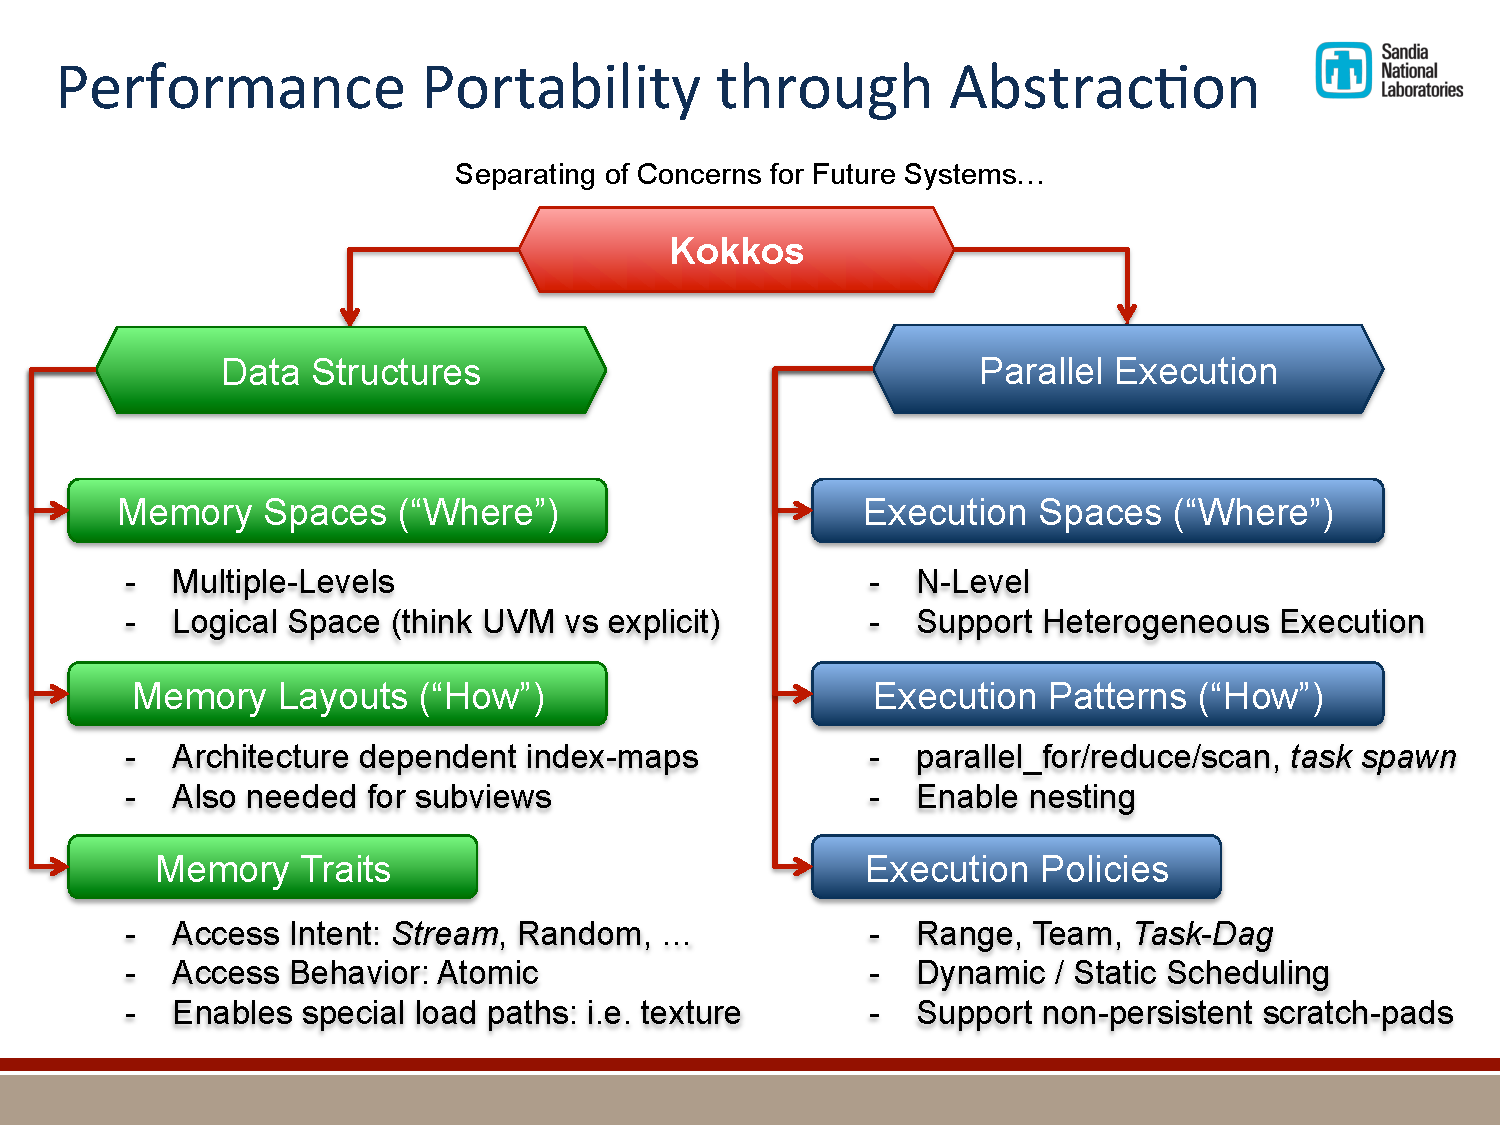
\includegraphics[width=8.5cm]{images/Kokkos-Multi-CoE_slide3}
  \end{center}

  {\small reference: \myurl{https://cfwebprod.sandia.gov/cfdocs/CompResearch/docs/Kokkos-Multi-CoE.pdf}}

\end{frame}

%%%%%%%%%%%%%%%%%%%%%%%%%%%%%%%%%%%%%%%%%%%%%%%%%%%%%%%%%%%%%%%%%%% 
%%%%%%%%%%%%%%%%%%%%%%%%%%%%%%%%%%%%%%%%%%%%%%%%%%%%%%%%%%%%%%%%%%% 
%%%%%%%%%%%%%%%%%%%%%%%%%%%%%%%%%%%%%%%%%%%%%%%%%%%%%%%%%%%%%%%%%%% 
\begin{frame}
  \frametitle{Kokkos: Sparse Matrix-Vector Multiply}

  \begin{center}
    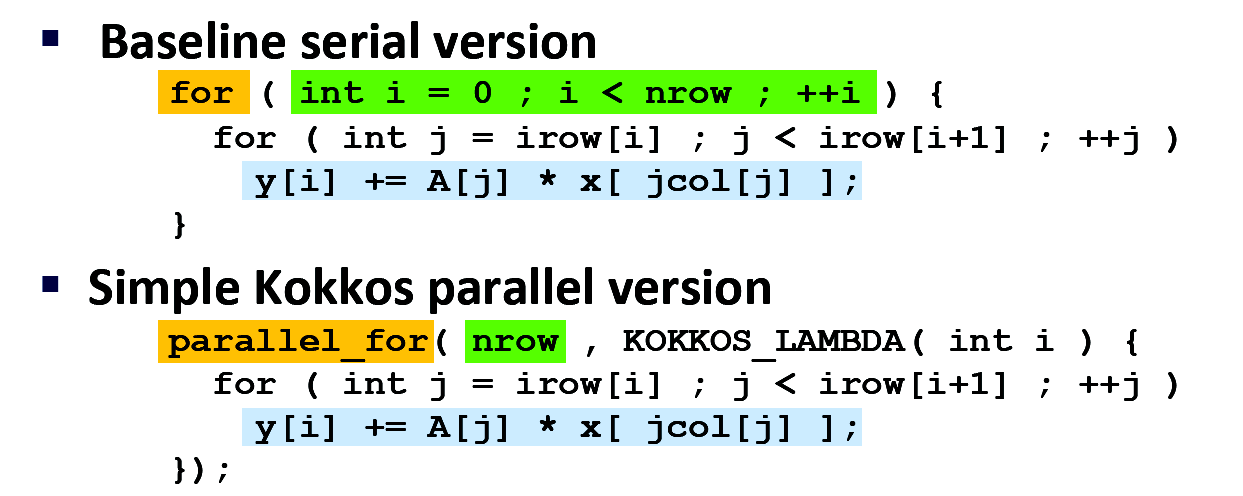
\includegraphics[width=8.5cm]{doc/perf_portability/kokkos_spmv}
  \end{center}

  \begin{itemize}
  \item Execution pattern: \textcolor{orange}{\textbf{parallel for}}
  \item Execution policy: \textcolor{darkgreen}{\textbf{range iteration}}
  \item Execution space: default (defined at compiled time)
  \item \textcolor{cyan}{\textbf{Work to do can be}}
    \begin{itemize}
    \item A \textbf{Lambda \textit{anonymous} function}, convenient for short loop bodies
    \item A \textbf{C++ class functor}, maximun flexibility
    \end{itemize}
  \end{itemize}
\end{frame}


%%%%%%%%%%%%%%%%%%%%%%%%%%%%%%%%%%%%%%%%%%%%%%%%%%%%%%%%%%%%%%%%%%% 
%%%%%%%%%%%%%%%%%%%%%%%%%%%%%%%%%%%%%%%%%%%%%%%%%%%%%%%%%%%%%%%%%%% 
%%%%%%%%%%%%%%%%%%%%%%%%%%%%%%%%%%%%%%%%%%%%%%%%%%%%%%%%%%%%%%%%%%% 
% \begin{frame}
%   \frametitle{Kokkos: a programming model for performance portability}
% \end{frame}

%%%%%%%%%%%%%%%%%%%%%%%%%%%%%%%%%%%%%%%%%%%%%%%%%%%%%%%%%%%%%%%%%%% 
%%%%%%%%%%%%%%%%%%%%%%%%%%%%%%%%%%%%%%%%%%%%%%%%%%%%%%%%%%%%%%%%%%% 
%%%%%%%%%%%%%%%%%%%%%%%%%%%%%%%%%%%%%%%%%%%%%%%%%%%%%%%%%%%%%%%%%%% 
% \begin{frame}
%   \frametitle{Future of accelerator programming: Kokkos among other}

%   \begin{center}
%     \includegraphics[width=8cm]{images/kokkos1}
%   \end{center}

%   {\scriptsize
%   reference: slides by Edwards, Trott, Sunderland (SANDIA) at GTC2014
%   \myhref{http://on-demand.gputechconf.com/gtc/2014/presentations/S4213-kokkos-manycore-device-perf-portability-library-hpc-apps.pdf}{Kokkos, a Manycore Device Performance Portability Library for C++ HPC Applications}}

% \end{frame}

%%%%%%%%%%%%%%%%%%%%%%%%%%%%%%%%%%%%%%%%%%%%%%%%%%%%%%%%%%%%%%%%%%% 
%%%%%%%%%%%%%%%%%%%%%%%%%%%%%%%%%%%%%%%%%%%%%%%%%%%%%%%%%%%%%%%%%%% 
%%%%%%%%%%%%%%%%%%%%%%%%%%%%%%%%%%%%%%%%%%%%%%%%%%%%%%%%%%%%%%%%%%% 
% \begin{frame}
%   \frametitle{Future of accelerator programming: Kokkos among other}

%   \begin{itemize}
%   \item kokkos multi-dimensional array\\
%     map multi-index $(i,j,k,...)$ $\Longleftrightarrow$ memory location in a \textbf{memory space}~\footnote{In the same line of idea, see chapter 28 of book \textit{High Performance Parallelism Pearls}, Morton order improve performance}
%   \item Kokkos will choose a default memory layout adapted to the target device
%   \item Decouple logical index $(i,j,k,...)$ from actual memory layout
%   \end{itemize}

% \end{frame}

%%%%%%%%%%%%%%%%%%%%%%%%%%%%%%%%%%%%%%%%%%%%%%%%%%%%%%%%%%%%%%%%%%% 
%%%%%%%%%%%%%%%%%%%%%%%%%%%%%%%%%%%%%%%%%%%%%%%%%%%%%%%%%%%%%%%%%%% 
%%%%%%%%%%%%%%%%%%%%%%%%%%%%%%%%%%%%%%%%%%%%%%%%%%%%%%%%%%%%%%%%%%% 
\begin{frame}
  \frametitle{Future of accelerator programming: Kokkos among other}

  MiniMD used to bench thread-scalable algorithm before integrating them 
  in LAMMPS (2014)

  \begin{center}
    \includegraphics<1>[height=5.0cm]{images/kokkos_minimd}
    %\includegraphics<2>[height=6.5cm]{images/kokkos_minimd2}
    \includegraphics<2>[height=4.0cm]{doc/perf_portability/stan_table_lj.png}
  \end{center}

  source:  \myurl{http://lammps.sandia.gov/bench.html}\\
  \myhref{http://lammps.sandia.gov/}{LAMMPS} Accelerator benchmarks for CPU, GPU, KNL  Oct 2016 

\end{frame}

